% tikzpic.teP
\documentclass[crop,tikz]{standalone}% 'crop' is the default for v1.0, before it was 'preview'

%Packages
\usepackage{xcolor}

%tikz libraries}}
\usetikzlibrary{shapes.geometric}

%Colors
\definecolor{susceptible}{RGB}{141,160,203}
\definecolor{recovery}{RGB}{102,194,165}
\definecolor{infection}{RGB}{252,141,98}
% \definecolor{intervention}{RGB}{231,138,195}
\definecolor{intervention}{RGB}{160, 120, 120}
\definecolor{nothing}{RGB}{225,225,225}

%New commands
\newcommand{\Leftscissor}{\large  X}
\newcommand{\Largescissor}{\Huge  X}

% Formatting macros:
\tikzstyle{node}=[minimum size= .5in,circle, draw]
\tikzset{intervened node fill/.style  args={#1,#2}{node,circle split part fill={#1,#2}}}


\tikzstyle{edge}=[diamond, draw]
\tikzstyle{intervention}=[fill = intervention]
\tikzstyle{contact}=[fill = infection]
\tikzstyle{recovery}=[fill = recovery]

\makeatletter
\tikzset{circle split part fill/.style  args={#1,#2}{%
    alias=tmp@name, % Jake's idea !!
    postaction={%
      insert path={
        \pgfextra{%
          \pgfpointdiff{\pgfpointanchor{\pgf@node@name}{center}}%
          {\pgfpointanchor{\pgf@node@name}{north}}%
          \pgfmathsetmacro\scale{1}
          \pgfmathsetmacro\insiderad{\pgf@y*\scale}
          \fill[#1] (\pgf@node@name.base) ([yshift=-\pgflinewidth]\pgf@node@name.north) arc
          (90:270:\insiderad-\pgflinewidth)--cycle;
          \fill[#2] (\pgf@node@name.base) ([yshift=\pgflinewidth]\pgf@node@name.south)  arc
          (270:450:\insiderad-\pgflinewidth)--cycle;            %  \end{scope}
        }}}}}
 \makeatother  
 
 \makeatletter
\tikzset{circle tri split part fill/.style  args={#1,#2,#3}{%
    alias=tmp@name, % Jake's idea !!
    postaction={%
      insert path={
        \pgfextra{%
          \pgfpointdiff{\pgfpointanchor{\pgf@node@name}{center}}%
          {\pgfpointanchor{\pgf@node@name}{north}}%
          \pgfmathsetmacro\scale{1}
          \pgfmathsetmacro\insiderad{\pgf@y*\scale}
          \fill[#1] (\pgf@node@name.base) ([yshift=-\pgflinewidth]\pgf@node@name.north) arc
          (90:210:\insiderad-\pgflinewidth)--(\pgf@node@name.center)--cycle;
          \fill[#2] (\pgf@node@name.base) ([yshift=-\pgflinewidth]\pgf@node@name.north)  arc
          (90:-30:\insiderad-\pgflinewidth)--(\pgf@node@name.center)--cycle; 
          \fill[#3] (\pgf@node@name.base) ([yshift=\pgflinewidth]\pgf@node@name.south)  arc
          (-90:-30:\insiderad-\pgflinewidth)--(\pgf@node@name.center)--cycle; 
          \fill[#3] (\pgf@node@name.base) ([yshift=\pgflinewidth]\pgf@node@name.south)  arc
          (270:210:\insiderad-\pgflinewidth)--(\pgf@node@name.center)--cycle;            %  \end{scope}
        }}}}}
 \makeatother

\begin{document}

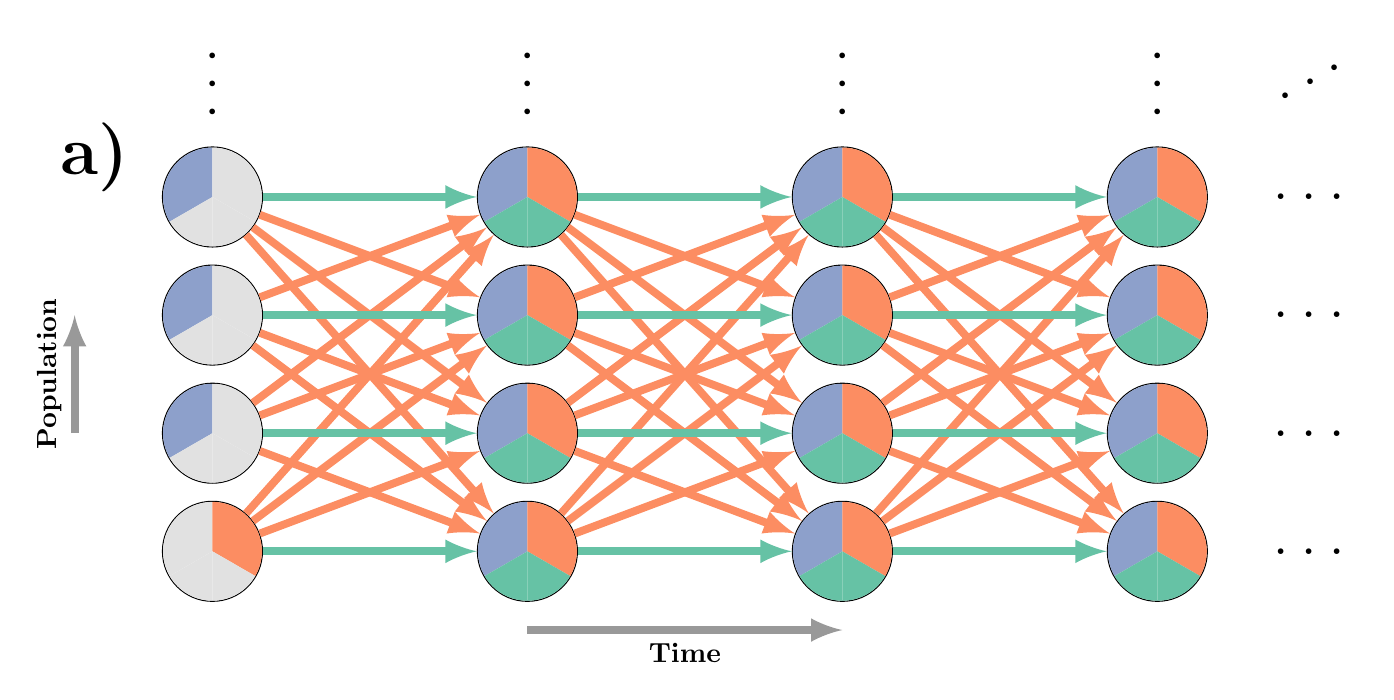
\begin{tikzpicture}
  \draw (-1.5,5) node {\Huge \textbf{a)}};

  \draw (0,0) node[node,circle tri split part fill={nothing,infection,nothing}] (P11) {};
  \draw (0,1.5) node[node,circle tri split part fill={susceptible,nothing,nothing}] (P21) {};
  \draw (0,3) node[node,circle tri split part fill={susceptible,nothing,nothing}] (P31) {};
  \draw (0,4.5) node[node,circle tri split part fill={susceptible,nothing,nothing}] (P41) {};

  \draw (4,0) node[node,circle tri split part fill={susceptible,infection,recovery}] (P12) {};
  \draw (4,1.5) node[node,circle tri split part fill={susceptible,infection,recovery}] (P22) {};
  \draw (4,3) node[node,circle tri split part fill={susceptible,infection,recovery}] (P32) {};
  \draw (4,4.5) node[node,circle tri split part fill={susceptible,infection,recovery}] (P42) {};

  \draw (8,0) node[node,circle tri split part fill={susceptible,infection,recovery}] (P13) {};
  \draw (8,1.5) node[node,circle tri split part fill={susceptible,infection,recovery}] (P23) {};
  \draw (8,3) node[node,circle tri split part fill={susceptible,infection,recovery}] (P33) {};
  \draw (8,4.5) node[node,circle tri split part fill={susceptible,infection,recovery}] (P43) {};

  \draw (12,0) node[node,circle tri split part fill={susceptible,infection,recovery}] (P14) {};
  \draw (12,1.5) node[node,circle tri split part fill={susceptible,infection,recovery}] (P24) {};
  \draw (12,3) node[node,circle tri split part fill={susceptible,infection,recovery}] (P34) {};
  \draw (12,4.5) node[node,circle tri split part fill={susceptible,infection,recovery}] (P44) {};

  \draw[-latex,line width=1mm, color=infection] (P11) -- (P22);
  \draw[-latex,line width=1mm, color=infection] (P11) -- (P32);
  \draw[-latex,line width=1mm, color=infection] (P11) -- (P42);
  \draw[-latex,line width=1mm, color=infection] (P21) -- (P12);
  \draw[-latex,line width=1mm, color=infection] (P21) -- (P32);
  \draw[-latex,line width=1mm, color=infection] (P21) -- (P42);
  \draw[-latex,line width=1mm, color=infection] (P31) -- (P12);
  \draw[-latex,line width=1mm, color=infection] (P31) -- (P22);
  \draw[-latex,line width=1mm, color=infection] (P31) -- (P42);
  \draw[-latex,line width=1mm, color=infection] (P41) -- (P12);
  \draw[-latex,line width=1mm, color=infection] (P41) -- (P22);
  \draw[-latex,line width=1mm, color=infection] (P41) -- (P32);
  
  \draw[-latex,line width=1mm, color=recovery] (P11) -- (P12);
  \draw[-latex,line width=1mm, color=recovery] (P21) -- (P22);
  \draw[-latex,line width=1mm, color=recovery] (P31) -- (P32);
  \draw[-latex,line width=1mm, color=recovery] (P41) -- (P42);
  
  \draw[-latex,line width=1mm, color=infection] (P12) -- (P23);
  \draw[-latex,line width=1mm, color=infection] (P12) -- (P33);
  \draw[-latex,line width=1mm, color=infection] (P12) -- (P43);
  \draw[-latex,line width=1mm, color=infection] (P22) -- (P13);
  \draw[-latex,line width=1mm, color=infection] (P22) -- (P33);
  \draw[-latex,line width=1mm, color=infection] (P22) -- (P43);
  \draw[-latex,line width=1mm, color=infection] (P32) -- (P13);
  \draw[-latex,line width=1mm, color=infection] (P32) -- (P23);
  \draw[-latex,line width=1mm, color=infection] (P32) -- (P43);
  \draw[-latex,line width=1mm, color=infection] (P42) -- (P13);
  \draw[-latex,line width=1mm, color=infection] (P42) -- (P23);
  \draw[-latex,line width=1mm, color=infection] (P42) -- (P33);
  
  \draw[-latex,line width=1mm, color=recovery] (P12) -- (P13);
  \draw[-latex,line width=1mm, color=recovery] (P22) -- (P23);
  \draw[-latex,line width=1mm, color=recovery] (P32) -- (P33);
  \draw[-latex,line width=1mm, color=recovery] (P42) -- (P43);
  
  \draw[-latex,line width=1mm, color=infection] (P13) -- (P24);
  \draw[-latex,line width=1mm, color=infection] (P13) -- (P34);
  \draw[-latex,line width=1mm, color=infection] (P13) -- (P44);
  \draw[-latex,line width=1mm, color=infection] (P23) -- (P14);
  \draw[-latex,line width=1mm, color=infection] (P23) -- (P34);
  \draw[-latex,line width=1mm, color=infection] (P23) -- (P44);
  \draw[-latex,line width=1mm, color=infection] (P33) -- (P14);
  \draw[-latex,line width=1mm, color=infection] (P33) -- (P24);
  \draw[-latex,line width=1mm, color=infection] (P33) -- (P44);
  \draw[-latex,line width=1mm, color=infection] (P43) -- (P14);
  \draw[-latex,line width=1mm, color=infection] (P43) -- (P24);
  \draw[-latex,line width=1mm, color=infection] (P43) -- (P34);
  
  \draw[-latex,line width=1mm, color=recovery] (P13) -- (P14);
  \draw[-latex,line width=1mm, color=recovery] (P23) -- (P24);
  \draw[-latex,line width=1mm, color=recovery] (P33) -- (P34);
  \draw[-latex,line width=1mm, color=recovery] (P43) -- (P44);

  %% Extends on
  \draw (14,0) node{\Huge \dots};
  \draw (14,1.5) node{\Huge \dots};
  \draw (14,3) node{\Huge \dots};
  \draw (14,4.5) node{\Huge \dots};

  \draw (0,6) node[rotate=90]{\Huge \dots};
  \draw (4,6) node[rotate=90]{\Huge \dots};
  \draw (8,6) node[rotate=90]{\Huge \dots};
  \draw (12,6) node[rotate=90]{\Huge \dots};
  \draw (14,6) node[rotate=30]{\Huge \dots};
  %% Legend things
  \draw[-latex,line width=1mm,white!60!black] (4,-1) -- (8,-1) node[midway, below,text=black] {\textbf{Time}};
  \draw[-latex,line width=1mm,white!60!black] (-1.75,1.5) -- (-1.75,3) node[midway, above,text=black,rotate=90] {\textbf{Population}};
\end{tikzpicture}

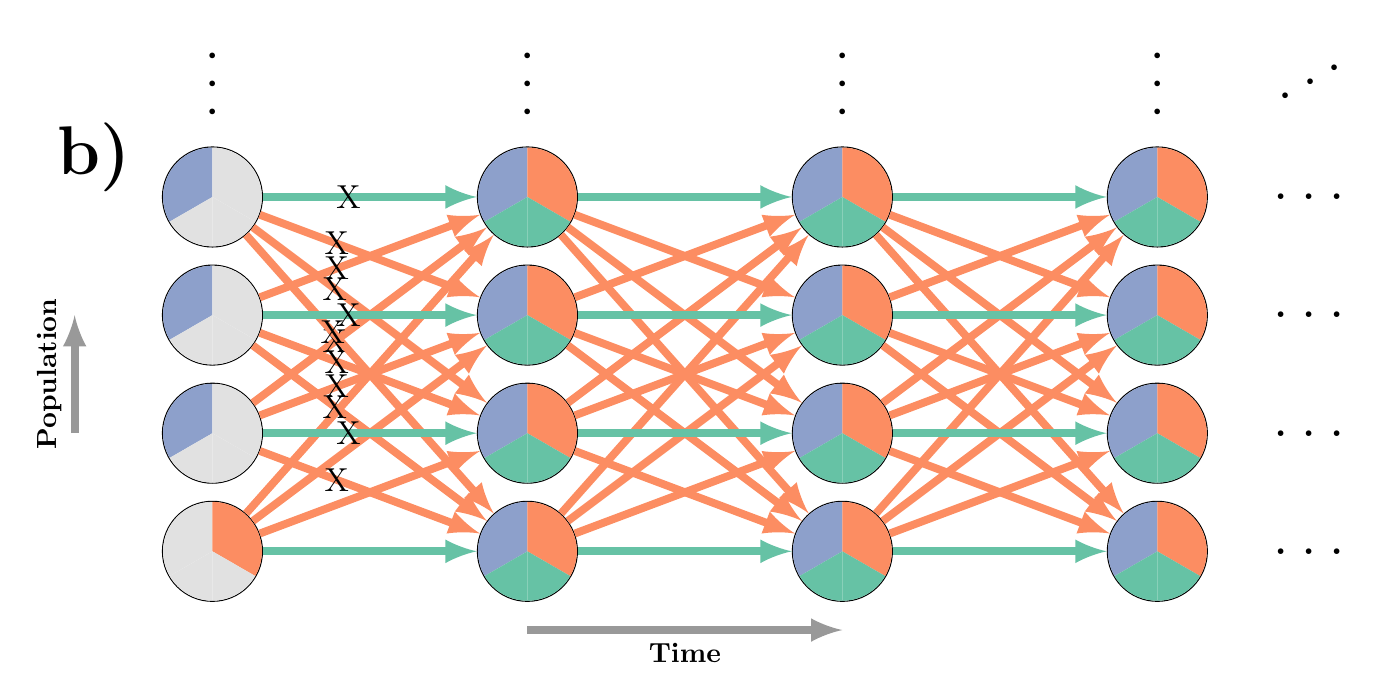
\begin{tikzpicture}
  \draw (-1.5,5) node {\Huge \textbf{b)}};
  \draw (0,0) node[node,circle tri split part fill={nothing,infection,nothing}] (P11) {};
  \draw (0,1.5) node[node,circle tri split part fill={susceptible,nothing,nothing}] (P21) {};
  \draw (0,3) node[node,circle tri split part fill={susceptible,nothing,nothing}] (P31) {};
  \draw (0,4.5) node[node,circle tri split part fill={susceptible,nothing,nothing}] (P41) {};

  \draw (4,0) node[node,circle tri split part fill={susceptible,infection,recovery}] (P12) {};
  \draw (4,1.5) node[node,circle tri split part fill={susceptible,infection,recovery}] (P22) {};
  \draw (4,3) node[node,circle tri split part fill={susceptible,infection,recovery}] (P32) {};
  \draw (4,4.5) node[node,circle tri split part fill={susceptible,infection,recovery}] (P42) {};

  \draw (8,0) node[node,circle tri split part fill={susceptible,infection,recovery}] (P13) {};
  \draw (8,1.5) node[node,circle tri split part fill={susceptible,infection,recovery}] (P23) {};
  \draw (8,3) node[node,circle tri split part fill={susceptible,infection,recovery}] (P33) {};
  \draw (8,4.5) node[node,circle tri split part fill={susceptible,infection,recovery}] (P43) {};

  \draw (12,0) node[node,circle tri split part fill={susceptible,infection,recovery}] (P14) {};
  \draw (12,1.5) node[node,circle tri split part fill={susceptible,infection,recovery}] (P24) {};
  \draw (12,3) node[node,circle tri split part fill={susceptible,infection,recovery}] (P34) {};
  \draw (12,4.5) node[node,circle tri split part fill={susceptible,infection,recovery}] (P44) {};

  \draw[-latex,line width=1mm, color=infection] (P11) -- (P22);
  \draw[-latex,line width=1mm, color=infection] (P11) -- (P32);
  \draw[-latex,line width=1mm, color=infection] (P11) -- (P42);
  \draw[-latex,line width=1mm, color=infection] (P21) --node[pos=.35,text=black]{\Leftscissor} (P12);
  \draw[-latex,line width=1mm, color=infection] (P21) --node[pos=.35,text=black]{\Leftscissor} (P32);
  \draw[-latex,line width=1mm, color=infection] (P21) --node[pos=.35,text=black]{\Leftscissor} (P42);
  \draw[-latex,line width=1mm, color=infection] (P31) --node[pos=.35,text=black]{\Leftscissor} (P12);
  \draw[-latex,line width=1mm, color=infection] (P31) --node[pos=.35,text=black]{\Leftscissor} (P22);
  \draw[-latex,line width=1mm, color=infection] (P31) --node[pos=.35,text=black]{\Leftscissor} (P42);
  \draw[-latex,line width=1mm, color=infection] (P41) --node[pos=.35,text=black]{\Leftscissor} (P12);
  \draw[-latex,line width=1mm, color=infection] (P41) --node[pos=.35,text=black]{\Leftscissor} (P22);
  \draw[-latex,line width=1mm, color=infection] (P41) --node[pos=.35,text=black]{\Leftscissor} (P32);
  
  \draw[-latex,line width=1mm, color=recovery] (P11) -- (P12);
  \draw[-latex,line width=1mm, color=recovery] (P21) --node[pos=.4,text=black]{\Leftscissor} (P22);
  \draw[-latex,line width=1mm, color=recovery] (P31) --node[pos=.4,text=black]{\Leftscissor} (P32);
  \draw[-latex,line width=1mm, color=recovery] (P41) --node[pos=.4,text=black]{\Leftscissor} (P42);
  
  \draw[-latex,line width=1mm, color=infection] (P12) -- (P23);
  \draw[-latex,line width=1mm, color=infection] (P12) -- (P33);
  \draw[-latex,line width=1mm, color=infection] (P12) -- (P43);
  \draw[-latex,line width=1mm, color=infection] (P22) -- (P13);
  \draw[-latex,line width=1mm, color=infection] (P22) -- (P33);
  \draw[-latex,line width=1mm, color=infection] (P22) -- (P43);
  \draw[-latex,line width=1mm, color=infection] (P32) -- (P13);
  \draw[-latex,line width=1mm, color=infection] (P32) -- (P23);
  \draw[-latex,line width=1mm, color=infection] (P32) -- (P43);
  \draw[-latex,line width=1mm, color=infection] (P42) -- (P13);
  \draw[-latex,line width=1mm, color=infection] (P42) -- (P23);
  \draw[-latex,line width=1mm, color=infection] (P42) -- (P33);
  
  \draw[-latex,line width=1mm, color=recovery] (P12) -- (P13);
  \draw[-latex,line width=1mm, color=recovery] (P22) -- (P23);
  \draw[-latex,line width=1mm, color=recovery] (P32) -- (P33);
  \draw[-latex,line width=1mm, color=recovery] (P42) -- (P43);
  
  \draw[-latex,line width=1mm, color=infection] (P13) -- (P24);
  \draw[-latex,line width=1mm, color=infection] (P13) -- (P34);
  \draw[-latex,line width=1mm, color=infection] (P13) -- (P44);
  \draw[-latex,line width=1mm, color=infection] (P23) -- (P14);
  \draw[-latex,line width=1mm, color=infection] (P23) -- (P34);
  \draw[-latex,line width=1mm, color=infection] (P23) -- (P44);
  \draw[-latex,line width=1mm, color=infection] (P33) -- (P14);
  \draw[-latex,line width=1mm, color=infection] (P33) -- (P24);
  \draw[-latex,line width=1mm, color=infection] (P33) -- (P44);
  \draw[-latex,line width=1mm, color=infection] (P43) -- (P14);
  \draw[-latex,line width=1mm, color=infection] (P43) -- (P24);
  \draw[-latex,line width=1mm, color=infection] (P43) -- (P34);
  
  \draw[-latex,line width=1mm, color=recovery] (P13) -- (P14);
  \draw[-latex,line width=1mm, color=recovery] (P23) -- (P24);
  \draw[-latex,line width=1mm, color=recovery] (P33) -- (P34);
  \draw[-latex,line width=1mm, color=recovery] (P43) -- (P44);

  %% Extends on
  \draw (14,0) node{\Huge \dots};
  \draw (14,1.5) node{\Huge \dots};
  \draw (14,3) node{\Huge \dots};
  \draw (14,4.5) node{\Huge \dots};

  \draw (0,6) node[rotate=90]{\Huge \dots};
  \draw (4,6) node[rotate=90]{\Huge \dots};
  \draw (8,6) node[rotate=90]{\Huge \dots};
  \draw (12,6) node[rotate=90]{\Huge \dots};
  \draw (14,6) node[rotate=30]{\Huge \dots};
  %% Legend things
  \draw[-latex,line width=1mm,white!60!black] (4,-1) -- (8,-1) node[midway, below,text=black] {\textbf{Time}};
  \draw[-latex,line width=1mm,white!60!black] (-1.75,1.5) -- (-1.75,3) node[midway, above,text=black,rotate=90] {\textbf{Population}};
\end{tikzpicture}

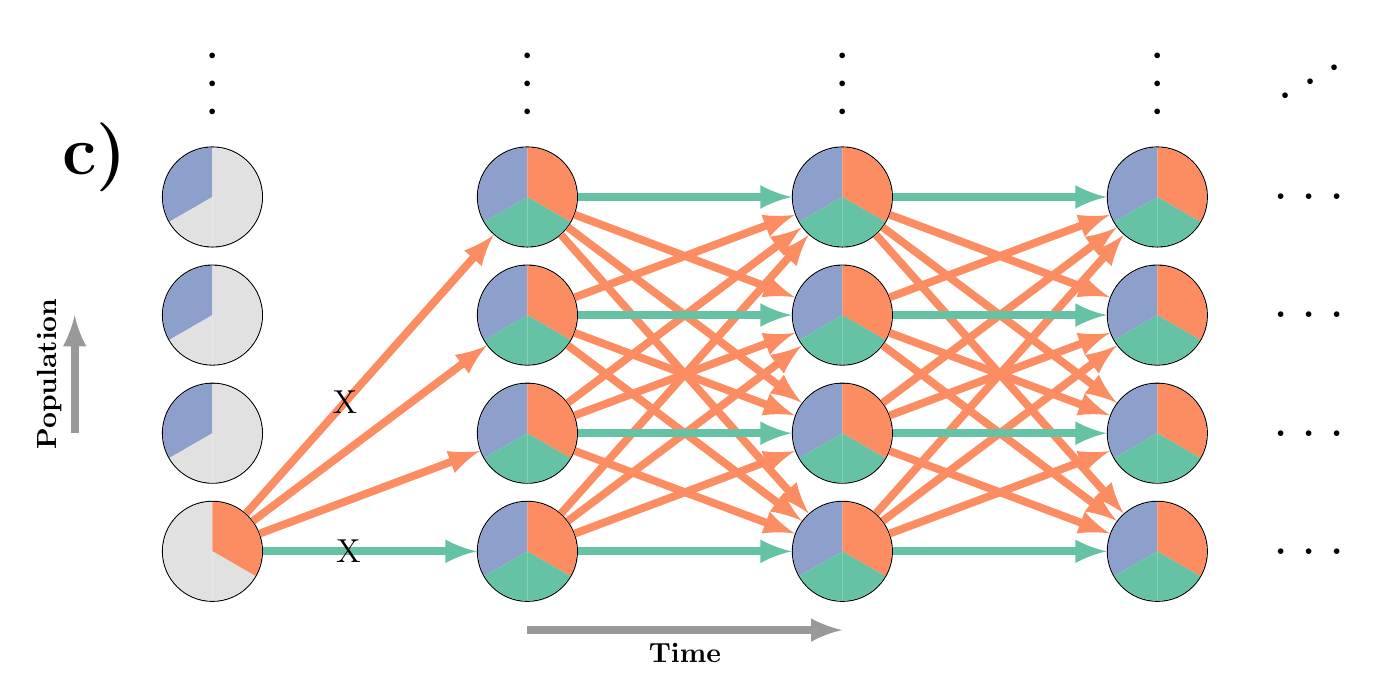
\begin{tikzpicture}
  \draw (-1.5,5) node {\Huge \textbf{c)}};
  \draw (0,0) node[node,circle tri split part fill={nothing,infection,nothing}] (P11) {};
  \draw (0,1.5) node[node,circle tri split part fill={susceptible,nothing,nothing}] (P21) {};
  \draw (0,3) node[node,circle tri split part fill={susceptible,nothing,nothing}] (P31) {};
  \draw (0,4.5) node[node,circle tri split part fill={susceptible,nothing,nothing}] (P41) {};

  \draw (4,0) node[node,circle tri split part fill={susceptible,infection,recovery}] (P12) {};
  \draw (4,1.5) node[node,circle tri split part fill={susceptible,infection,recovery}] (P22) {};
  \draw (4,3) node[node,circle tri split part fill={susceptible,infection,recovery}] (P32) {};
  \draw (4,4.5) node[node,circle tri split part fill={susceptible,infection,recovery}] (P42) {};

  \draw (8,0) node[node,circle tri split part fill={susceptible,infection,recovery}] (P13) {};
  \draw (8,1.5) node[node,circle tri split part fill={susceptible,infection,recovery}] (P23) {};
  \draw (8,3) node[node,circle tri split part fill={susceptible,infection,recovery}] (P33) {};
  \draw (8,4.5) node[node,circle tri split part fill={susceptible,infection,recovery}] (P43) {};

  \draw (12,0) node[node,circle tri split part fill={susceptible,infection,recovery}] (P14) {};
  \draw (12,1.5) node[node,circle tri split part fill={susceptible,infection,recovery}] (P24) {};
  \draw (12,3) node[node,circle tri split part fill={susceptible,infection,recovery}] (P34) {};
  \draw (12,4.5) node[node,circle tri split part fill={susceptible,infection,recovery}] (P44) {};

  \draw[-latex,line width=1mm, color=infection] (P11) -- (P22);
  \draw[-latex,line width=1mm, color=infection] (P11) -- (P32);
  \draw[-latex,line width=1mm, color=infection] (P11) --node[pos=.4,text=black]{\Leftscissor} (P42);
  
  \draw[-latex,line width=1mm, color=recovery] (P11) --node[pos=.4,text=black]{\Leftscissor} (P12);
  
  \draw[-latex,line width=1mm, color=infection] (P12) -- (P23);
  \draw[-latex,line width=1mm, color=infection] (P12) -- (P33);
  \draw[-latex,line width=1mm, color=infection] (P12) -- (P43);
  \draw[-latex,line width=1mm, color=infection] (P22) -- (P13);
  \draw[-latex,line width=1mm, color=infection] (P22) -- (P33);
  \draw[-latex,line width=1mm, color=infection] (P22) -- (P43);
  \draw[-latex,line width=1mm, color=infection] (P32) -- (P13);
  \draw[-latex,line width=1mm, color=infection] (P32) -- (P23);
  \draw[-latex,line width=1mm, color=infection] (P32) -- (P43);
  \draw[-latex,line width=1mm, color=infection] (P42) -- (P13);
  \draw[-latex,line width=1mm, color=infection] (P42) -- (P23);
  \draw[-latex,line width=1mm, color=infection] (P42) -- (P33);
  
  \draw[-latex,line width=1mm, color=recovery] (P12) -- (P13);
  \draw[-latex,line width=1mm, color=recovery] (P22) -- (P23);
  \draw[-latex,line width=1mm, color=recovery] (P32) -- (P33);
  \draw[-latex,line width=1mm, color=recovery] (P42) -- (P43);
  
  \draw[-latex,line width=1mm, color=infection] (P13) -- (P24);
  \draw[-latex,line width=1mm, color=infection] (P13) -- (P34);
  \draw[-latex,line width=1mm, color=infection] (P13) -- (P44);
  \draw[-latex,line width=1mm, color=infection] (P23) -- (P14);
  \draw[-latex,line width=1mm, color=infection] (P23) -- (P34);
  \draw[-latex,line width=1mm, color=infection] (P23) -- (P44);
  \draw[-latex,line width=1mm, color=infection] (P33) -- (P14);
  \draw[-latex,line width=1mm, color=infection] (P33) -- (P24);
  \draw[-latex,line width=1mm, color=infection] (P33) -- (P44);
  \draw[-latex,line width=1mm, color=infection] (P43) -- (P14);
  \draw[-latex,line width=1mm, color=infection] (P43) -- (P24);
  \draw[-latex,line width=1mm, color=infection] (P43) -- (P34);
  
  \draw[-latex,line width=1mm, color=recovery] (P13) -- (P14);
  \draw[-latex,line width=1mm, color=recovery] (P23) -- (P24);
  \draw[-latex,line width=1mm, color=recovery] (P33) -- (P34);
  \draw[-latex,line width=1mm, color=recovery] (P43) -- (P44);

  %% Extends on
  \draw (14,0) node{\Huge \dots};
  \draw (14,1.5) node{\Huge \dots};
  \draw (14,3) node{\Huge \dots};
  \draw (14,4.5) node{\Huge \dots};

  \draw (0,6) node[rotate=90]{\Huge \dots};
  \draw (4,6) node[rotate=90]{\Huge \dots};
  \draw (8,6) node[rotate=90]{\Huge \dots};
  \draw (12,6) node[rotate=90]{\Huge \dots};
  \draw (14,6) node[rotate=30]{\Huge \dots};
  %% Legend things
  \draw[-latex,line width=1mm,white!60!black] (4,-1) -- (8,-1) node[midway, below,text=black] {\textbf{Time}};
  \draw[-latex,line width=1mm,white!60!black] (-1.75,1.5) -- (-1.75,3) node[midway, above,text=black,rotate=90] {\textbf{Population}};
\end{tikzpicture}

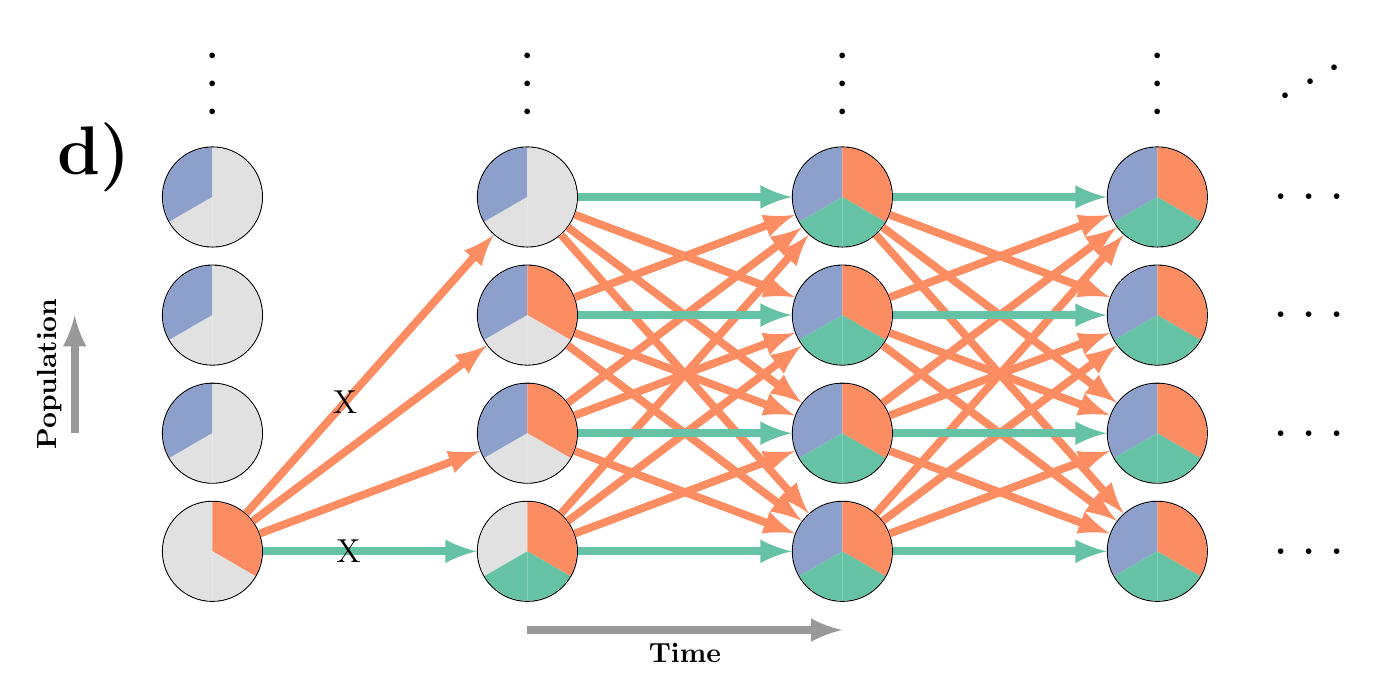
\begin{tikzpicture}
  \draw (-1.5,5) node {\Huge \textbf{d)}};
  \draw (0,0) node[node,circle tri split part fill={nothing,infection,nothing}] (P11) {};
  \draw (0,1.5) node[node,circle tri split part fill={susceptible,nothing,nothing}] (P21) {};
  \draw (0,3) node[node,circle tri split part fill={susceptible,nothing,nothing}] (P31) {};
  \draw (0,4.5) node[node,circle tri split part fill={susceptible,nothing,nothing}] (P41) {};

  \draw (4,0) node[node,circle tri split part fill={nothing,infection,recovery}] (P12) {};
  \draw (4,1.5) node[node,circle tri split part fill={susceptible,infection,nothing}] (P22) {};
  \draw (4,3) node[node,circle tri split part fill={susceptible,infection,nothing}] (P32) {};
  \draw (4,4.5) node[node,circle tri split part fill={susceptible,nothing,nothing}] (P42) {};

  \draw (8,0) node[node,circle tri split part fill={susceptible,infection,recovery}] (P13) {};
  \draw (8,1.5) node[node,circle tri split part fill={susceptible,infection,recovery}] (P23) {};
  \draw (8,3) node[node,circle tri split part fill={susceptible,infection,recovery}] (P33) {};
  \draw (8,4.5) node[node,circle tri split part fill={susceptible,infection,recovery}] (P43) {};

  \draw (12,0) node[node,circle tri split part fill={susceptible,infection,recovery}] (P14) {};
  \draw (12,1.5) node[node,circle tri split part fill={susceptible,infection,recovery}] (P24) {};
  \draw (12,3) node[node,circle tri split part fill={susceptible,infection,recovery}] (P34) {};
  \draw (12,4.5) node[node,circle tri split part fill={susceptible,infection,recovery}] (P44) {};

  \draw[-latex,line width=1mm, color=infection] (P11) -- (P22);
  \draw[-latex,line width=1mm, color=infection] (P11) -- (P32);
  \draw[-latex,line width=1mm, color=infection] (P11) -- node[pos=.4,text=black]{\Leftscissor} (P42);

  
  \draw[-latex,line width=1mm, color=recovery] (P11) -- node[pos=.4,text=black]{\Leftscissor} (P12);
  
  \draw[-latex,line width=1mm, color=infection] (P12) -- (P23);
  \draw[-latex,line width=1mm, color=infection] (P12) -- (P33);
  \draw[-latex,line width=1mm, color=infection] (P12) -- (P43);
  \draw[-latex,line width=1mm, color=infection] (P22) -- (P13);
  \draw[-latex,line width=1mm, color=infection] (P22) -- (P33);
  \draw[-latex,line width=1mm, color=infection] (P22) -- (P43);
  \draw[-latex,line width=1mm, color=infection] (P32) -- (P13);
  \draw[-latex,line width=1mm, color=infection] (P32) -- (P23);
  \draw[-latex,line width=1mm, color=infection] (P32) -- (P43);
  \draw[-latex,line width=1mm, color=infection] (P42) -- (P13);
  \draw[-latex,line width=1mm, color=infection] (P42) -- (P23);
  \draw[-latex,line width=1mm, color=infection] (P42) -- (P33);
  
  \draw[-latex,line width=1mm, color=recovery] (P12) -- (P13);
  \draw[-latex,line width=1mm, color=recovery] (P22) -- (P23);
  \draw[-latex,line width=1mm, color=recovery] (P32) -- (P33);
  \draw[-latex,line width=1mm, color=recovery] (P42) -- (P43);
  
  \draw[-latex,line width=1mm, color=infection] (P13) -- (P24);
  \draw[-latex,line width=1mm, color=infection] (P13) -- (P34);
  \draw[-latex,line width=1mm, color=infection] (P13) -- (P44);
  \draw[-latex,line width=1mm, color=infection] (P23) -- (P14);
  \draw[-latex,line width=1mm, color=infection] (P23) -- (P34);
  \draw[-latex,line width=1mm, color=infection] (P23) -- (P44);
  \draw[-latex,line width=1mm, color=infection] (P33) -- (P14);
  \draw[-latex,line width=1mm, color=infection] (P33) -- (P24);
  \draw[-latex,line width=1mm, color=infection] (P33) -- (P44);
  \draw[-latex,line width=1mm, color=infection] (P43) -- (P14);
  \draw[-latex,line width=1mm, color=infection] (P43) -- (P24);
  \draw[-latex,line width=1mm, color=infection] (P43) -- (P34);
  
  \draw[-latex,line width=1mm, color=recovery] (P13) -- (P14);
  \draw[-latex,line width=1mm, color=recovery] (P23) -- (P24);
  \draw[-latex,line width=1mm, color=recovery] (P33) -- (P34);
  \draw[-latex,line width=1mm, color=recovery] (P43) -- (P44);

  %% Extends on
  \draw (14,0) node{\Huge \dots};
  \draw (14,1.5) node{\Huge \dots};
  \draw (14,3) node{\Huge \dots};
  \draw (14,4.5) node{\Huge \dots};

  \draw (0,6) node[rotate=90]{\Huge \dots};
  \draw (4,6) node[rotate=90]{\Huge \dots};
  \draw (8,6) node[rotate=90]{\Huge \dots};
  \draw (12,6) node[rotate=90]{\Huge \dots};
  \draw (14,6) node[rotate=30]{\Huge \dots};
  %% Legend things
  \draw[-latex,line width=1mm,white!60!black] (4,-1) -- (8,-1) node[midway, below,text=black] {\textbf{Time}};
  \draw[-latex,line width=1mm,white!60!black] (-1.75,1.5) -- (-1.75,3) node[midway, above,text=black,rotate=90] {\textbf{Population}};
\end{tikzpicture}

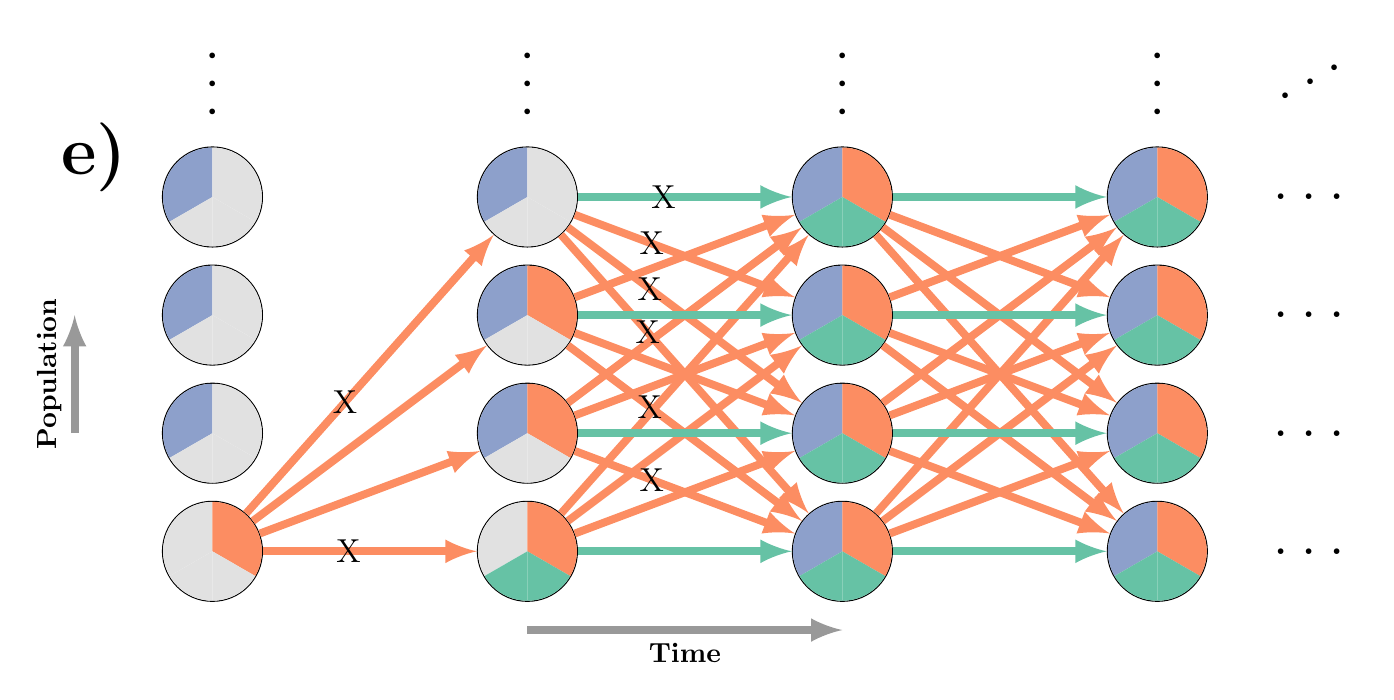
\begin{tikzpicture}
  \draw (-1.5,5) node {\Huge \textbf{e)}};
  \draw (0,0) node[node,circle tri split part fill={nothing,infection,nothing}] (P11) {};
  \draw (0,1.5) node[node,circle tri split part fill={susceptible,nothing,nothing}] (P21) {};
  \draw (0,3) node[node,circle tri split part fill={susceptible,nothing,nothing}] (P31) {};
  \draw (0,4.5) node[node,circle tri split part fill={susceptible,nothing,nothing}] (P41) {};

  \draw (4,0) node[node,circle tri split part fill={nothing,infection,recovery}] (P12) {};
  \draw (4,1.5) node[node,circle tri split part fill={susceptible,infection,nothing}] (P22) {};
  \draw (4,3) node[node,circle tri split part fill={susceptible,infection,nothing}] (P32) {};
  \draw (4,4.5) node[node,circle tri split part fill={susceptible,nothing,nothing}] (P42) {};

  \draw (8,0) node[node,circle tri split part fill={susceptible,infection,recovery}] (P13) {};
  \draw (8,1.5) node[node,circle tri split part fill={susceptible,infection,recovery}] (P23) {};
  \draw (8,3) node[node,circle tri split part fill={susceptible,infection,recovery}] (P33) {};
  \draw (8,4.5) node[node,circle tri split part fill={susceptible,infection,recovery}] (P43) {};

  \draw (12,0) node[node,circle tri split part fill={susceptible,infection,recovery}] (P14) {};
  \draw (12,1.5) node[node,circle tri split part fill={susceptible,infection,recovery}] (P24) {};
  \draw (12,3) node[node,circle tri split part fill={susceptible,infection,recovery}] (P34) {};
  \draw (12,4.5) node[node,circle tri split part fill={susceptible,infection,recovery}] (P44) {};

  \draw[-latex,line width=1mm, color=infection] (P11) -- (P22);
  \draw[-latex,line width=1mm, color=infection] (P11) -- (P32);
  \draw[-latex,line width=1mm, color=infection] (P11) --node[pos=.4,text=black]{\Leftscissor} (P42);

  
  \draw[-latex,line width=1mm, color=infection] (P11) --node[pos=.4,text=black]{\Leftscissor} (P12);
  
  \draw[-latex,line width=1mm, color=infection] (P12) -- (P23);
  \draw[-latex,line width=1mm, color=infection] (P12) -- (P33);
  \draw[-latex,line width=1mm, color=infection] (P12) -- (P43);
  \draw[-latex,line width=1mm, color=infection] (P22) -- node[pos=.35,text=black]{\Leftscissor} (P13);
  \draw[-latex,line width=1mm, color=infection] (P22) -- (P33);
  \draw[-latex,line width=1mm, color=infection] (P22) -- (P43);
  \draw[-latex,line width=1mm, color=infection] (P32) -- node[pos=.35,text=black]{\Leftscissor} (P13);
  \draw[-latex,line width=1mm, color=infection] (P32) -- (P23);
  \draw[-latex,line width=1mm, color=infection] (P32) -- (P43);
  \draw[-latex,line width=1mm, color=infection] (P42) -- node[pos=.35,text=black]{\Leftscissor} (P13);
  \draw[-latex,line width=1mm, color=infection] (P42) -- node[pos=.35,text=black]{\Leftscissor} (P23);
  \draw[-latex,line width=1mm, color=infection] (P42) -- node[pos=.35,text=black]{\Leftscissor} (P33);
  
  \draw[-latex,line width=1mm, color=recovery] (P12) -- (P13);
  \draw[-latex,line width=1mm, color=recovery] (P22) -- (P23);
  \draw[-latex,line width=1mm, color=recovery] (P32) -- (P33);
  \draw[-latex,line width=1mm, color=recovery] (P42) -- node[pos=.4,text=black]{\Leftscissor} (P43);
  
  \draw[-latex,line width=1mm, color=infection] (P13) -- (P24);
  \draw[-latex,line width=1mm, color=infection] (P13) -- (P34);
  \draw[-latex,line width=1mm, color=infection] (P13) -- (P44);
  \draw[-latex,line width=1mm, color=infection] (P23) -- (P14);
  \draw[-latex,line width=1mm, color=infection] (P23) -- (P34);
  \draw[-latex,line width=1mm, color=infection] (P23) -- (P44);
  \draw[-latex,line width=1mm, color=infection] (P33) -- (P14);
  \draw[-latex,line width=1mm, color=infection] (P33) -- (P24);
  \draw[-latex,line width=1mm, color=infection] (P33) -- (P44);
  \draw[-latex,line width=1mm, color=infection] (P43) -- (P14);
  \draw[-latex,line width=1mm, color=infection] (P43) -- (P24);
  \draw[-latex,line width=1mm, color=infection] (P43) -- (P34);
  
  \draw[-latex,line width=1mm, color=recovery] (P13) -- (P14);
  \draw[-latex,line width=1mm, color=recovery] (P23) -- (P24);
  \draw[-latex,line width=1mm, color=recovery] (P33) -- (P34);
  \draw[-latex,line width=1mm, color=recovery] (P43) -- (P44);

  %% Extends on
  \draw (14,0) node{\Huge \dots};
  \draw (14,1.5) node{\Huge \dots};
  \draw (14,3) node{\Huge \dots};
  \draw (14,4.5) node{\Huge \dots};

  \draw (0,6) node[rotate=90]{\Huge \dots};
  \draw (4,6) node[rotate=90]{\Huge \dots};
  \draw (8,6) node[rotate=90]{\Huge \dots};
  \draw (12,6) node[rotate=90]{\Huge \dots};
  \draw (14,6) node[rotate=30]{\Huge \dots};
  %% Legend things
  \draw[-latex,line width=1mm,white!60!black] (4,-1) -- (8,-1) node[midway, below,text=black] {\textbf{Time}};
  \draw[-latex,line width=1mm,white!60!black] (-1.75,1.5) -- (-1.75,3) node[midway, above,text=black,rotate=90] {\textbf{Population}};
\end{tikzpicture}

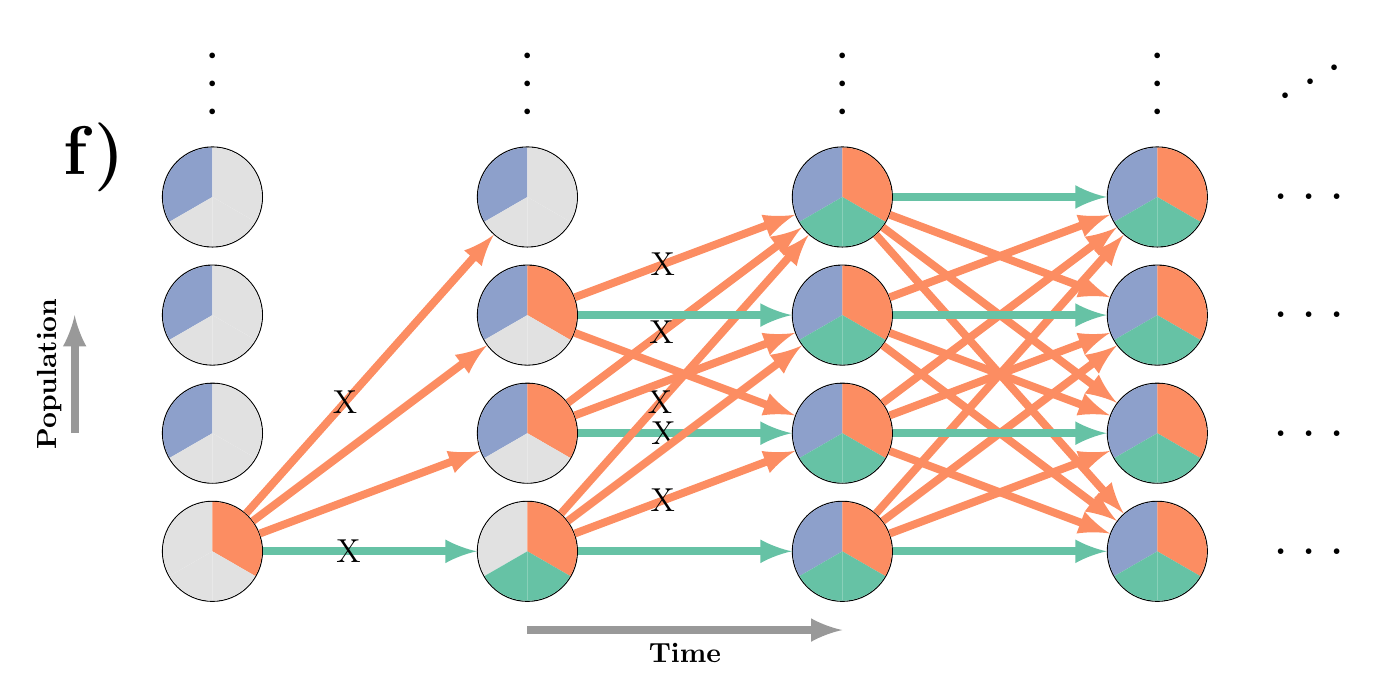
\begin{tikzpicture}
  \draw (-1.5,5) node {\Huge \textbf{f)}};
  \draw (0,0) node[node,circle tri split part fill={nothing,infection,nothing}] (P11) {};
  \draw (0,1.5) node[node,circle tri split part fill={susceptible,nothing,nothing}] (P21) {};
  \draw (0,3) node[node,circle tri split part fill={susceptible,nothing,nothing}] (P31) {};
  \draw (0,4.5) node[node,circle tri split part fill={susceptible,nothing,nothing}] (P41) {};

  \draw (4,0) node[node,circle tri split part fill={nothing,infection,recovery}] (P12) {};
  \draw (4,1.5) node[node,circle tri split part fill={susceptible,infection,nothing}] (P22) {};
  \draw (4,3) node[node,circle tri split part fill={susceptible,infection,nothing}] (P32) {};
  \draw (4,4.5) node[node,circle tri split part fill={susceptible,nothing,nothing}] (P42) {};

  \draw (8,0) node[node,circle tri split part fill={susceptible,infection,recovery}] (P13) {};
  \draw (8,1.5) node[node,circle tri split part fill={susceptible,infection,recovery}] (P23) {};
  \draw (8,3) node[node,circle tri split part fill={susceptible,infection,recovery}] (P33) {};
  \draw (8,4.5) node[node,circle tri split part fill={susceptible,infection,recovery}] (P43) {};

  \draw (12,0) node[node,circle tri split part fill={susceptible,infection,recovery}] (P14) {};
  \draw (12,1.5) node[node,circle tri split part fill={susceptible,infection,recovery}] (P24) {};
  \draw (12,3) node[node,circle tri split part fill={susceptible,infection,recovery}] (P34) {};
  \draw (12,4.5) node[node,circle tri split part fill={susceptible,infection,recovery}] (P44) {};

  \draw[-latex,line width=1mm, color=infection] (P11) -- node[pos=.4,text=black]{\Leftscissor} (P42);
  \draw[-latex,line width=1mm, color=infection] (P11) -- (P22);
  \draw[-latex,line width=1mm, color=infection] (P11) -- (P32);
  
  \draw[-latex,line width=1mm, color=recovery] (P11) -- node[pos=.4,text=black]{\Leftscissor} (P12);
  \draw[-latex,line width=1mm, color=recovery] (P22) --  node[pos=.4,text=black]{\Leftscissor}(P23);
  
  \draw[-latex,line width=1mm, color=infection] (P12) -- node[pos=.4,text=black]{\Leftscissor} (P23);
  \draw[-latex,line width=1mm, color=infection] (P12) -- node[pos=.4,text=black]{\Leftscissor} (P43);
  \draw[-latex,line width=1mm, color=infection] (P22) -- node[pos=.4,text=black]{\Leftscissor} (P43);
  \draw[-latex,line width=1mm, color=infection] (P32) -- node[pos=.4,text=black]{\Leftscissor} (P43);
  \draw[-latex,line width=1mm, color=infection] (P12) -- (P33);
  \draw[-latex,line width=1mm, color=infection] (P22) -- (P33);
  \draw[-latex,line width=1mm, color=infection] (P32) -- (P23);

  \draw[-latex,line width=1mm, color=recovery] (P12) -- (P13);
  \draw[-latex,line width=1mm, color=recovery] (P32) -- (P33);
  
  \draw[-latex,line width=1mm, color=infection] (P13) -- (P24);
  \draw[-latex,line width=1mm, color=infection] (P13) -- (P34);
  \draw[-latex,line width=1mm, color=infection] (P13) -- (P44);
  \draw[-latex,line width=1mm, color=infection] (P23) -- (P14);
  \draw[-latex,line width=1mm, color=infection] (P23) -- (P34);
  \draw[-latex,line width=1mm, color=infection] (P23) -- (P44);
  \draw[-latex,line width=1mm, color=infection] (P33) -- (P14);
  \draw[-latex,line width=1mm, color=infection] (P33) -- (P24);
  \draw[-latex,line width=1mm, color=infection] (P33) -- (P44);
  \draw[-latex,line width=1mm, color=infection] (P43) -- (P14);
  \draw[-latex,line width=1mm, color=infection] (P43) -- (P24);
  \draw[-latex,line width=1mm, color=infection] (P43) -- (P34);
  
  \draw[-latex,line width=1mm, color=recovery] (P13) -- (P14);
  \draw[-latex,line width=1mm, color=recovery] (P23) -- (P24);
  \draw[-latex,line width=1mm, color=recovery] (P33) -- (P34);
  \draw[-latex,line width=1mm, color=recovery] (P43) -- (P44);

  %% Extends on
  \draw (14,0) node{\Huge \dots};
  \draw (14,1.5) node{\Huge \dots};
  \draw (14,3) node{\Huge \dots};
  \draw (14,4.5) node{\Huge \dots};

  \draw (0,6) node[rotate=90]{\Huge \dots};
  \draw (4,6) node[rotate=90]{\Huge \dots};
  \draw (8,6) node[rotate=90]{\Huge \dots};
  \draw (12,6) node[rotate=90]{\Huge \dots};
  \draw (14,6) node[rotate=30]{\Huge \dots};
  %% Legend things
  \draw[-latex,line width=1mm,white!60!black] (4,-1) -- (8,-1) node[midway, below,text=black] {\textbf{Time}};
  \draw[-latex,line width=1mm,white!60!black] (-1.75,1.5) -- (-1.75,3) node[midway, above,text=black,rotate=90] {\textbf{Population}};
\end{tikzpicture}

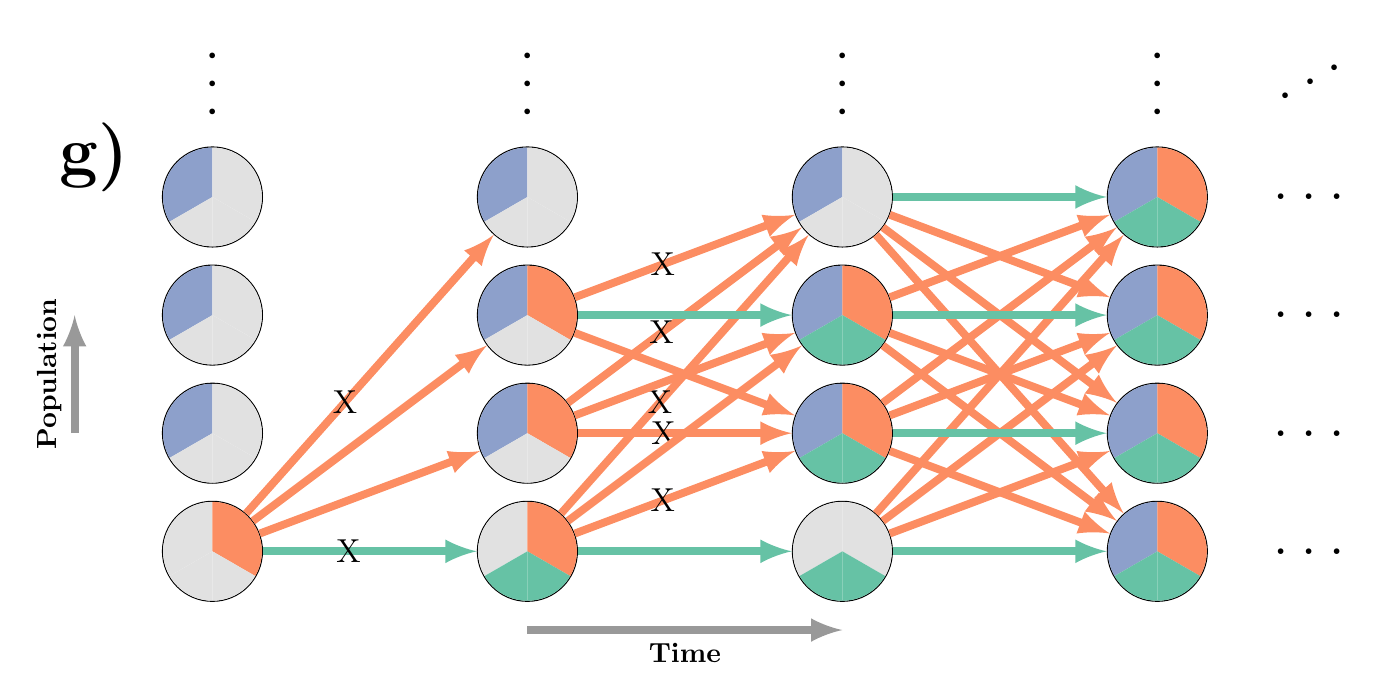
\begin{tikzpicture}
  \draw (-1.5,5) node {\Huge \textbf{g)}};
  \draw (0,0) node[node,circle tri split part fill={nothing,infection,nothing}] (P11) {};
  \draw (0,1.5) node[node,circle tri split part fill={susceptible,nothing,nothing}] (P21) {};
  \draw (0,3) node[node,circle tri split part fill={susceptible,nothing,nothing}] (P31) {};
  \draw (0,4.5) node[node,circle tri split part fill={susceptible,nothing,nothing}] (P41) {};

  \draw (4,0) node[node,circle tri split part fill={nothing,infection,recovery}] (P12) {};
  \draw (4,1.5) node[node,circle tri split part fill={susceptible,infection,nothing}] (P22) {};
  \draw (4,3) node[node,circle tri split part fill={susceptible,infection,nothing}] (P32) {};
  \draw (4,4.5) node[node,circle tri split part fill={susceptible,nothing,nothing}] (P42) {};

  \draw (8,0) node[node,circle tri split part fill={nothing,nothing,recovery}] (P13) {};
  \draw (8,1.5) node[node,circle tri split part fill={susceptible,infection,recovery}] (P23) {};
  \draw (8,3) node[node,circle tri split part fill={susceptible,infection,recovery}] (P33) {};
  \draw (8,4.5) node[node,circle tri split part fill={susceptible,nothing,nothing}] (P43) {};

  \draw (12,0) node[node,circle tri split part fill={susceptible,infection,recovery}] (P14) {};
  \draw (12,1.5) node[node,circle tri split part fill={susceptible,infection,recovery}] (P24) {};
  \draw (12,3) node[node,circle tri split part fill={susceptible,infection,recovery}] (P34) {};
  \draw (12,4.5) node[node,circle tri split part fill={susceptible,infection,recovery}] (P44) {};

  \draw[-latex,line width=1mm, color=infection] (P11) -- (P22);
  \draw[-latex,line width=1mm, color=infection] (P11) -- (P32);
  \draw[-latex,line width=1mm, color=infection] (P11) -- node[pos=.4,text=black]{\Leftscissor} (P42);
  
  \draw[-latex,line width=1mm, color=recovery] (P11) -- node[pos=.4,text=black]{\Leftscissor} (P12);
  
  \draw[-latex,line width=1mm, color=infection] (P12) -- node[pos=.4,text=black]{\Leftscissor} (P23);
  \draw[-latex,line width=1mm, color=infection] (P12) -- node[pos=.4,text=black]{\Leftscissor} (P43);
  \draw[-latex,line width=1mm, color=infection] (P22) -- node[pos=.4,text=black]{\Leftscissor} (P43);
  \draw[-latex,line width=1mm, color=infection] (P32) -- node[pos=.4,text=black]{\Leftscissor} (P43);
  \draw[-latex,line width=1mm, color=infection] (P22) -- node[pos=.4,text=black]{\Leftscissor} (P23);

  \draw[-latex,line width=1mm, color=infection] (P12) -- (P33);
  \draw[-latex,line width=1mm, color=infection] (P22) -- (P33);
  \draw[-latex,line width=1mm, color=infection] (P32) -- (P23);
  
  \draw[-latex,line width=1mm, color=recovery] (P12) -- (P13);
  \draw[-latex,line width=1mm, color=recovery] (P32) -- (P33);
  
  \draw[-latex,line width=1mm, color=infection] (P13) -- (P24);
  \draw[-latex,line width=1mm, color=infection] (P13) -- (P34);
  \draw[-latex,line width=1mm, color=infection] (P13) -- (P44);
  \draw[-latex,line width=1mm, color=infection] (P23) -- (P14);
  \draw[-latex,line width=1mm, color=infection] (P23) -- (P34);
  \draw[-latex,line width=1mm, color=infection] (P23) -- (P44);
  \draw[-latex,line width=1mm, color=infection] (P33) -- (P14);
  \draw[-latex,line width=1mm, color=infection] (P33) -- (P24);
  \draw[-latex,line width=1mm, color=infection] (P33) -- (P44);
  \draw[-latex,line width=1mm, color=infection] (P43) -- (P14);
  \draw[-latex,line width=1mm, color=infection] (P43) -- (P24);
  \draw[-latex,line width=1mm, color=infection] (P43) -- (P34);
  
  \draw[-latex,line width=1mm, color=recovery] (P13) -- (P14);
  \draw[-latex,line width=1mm, color=recovery] (P23) -- (P24);
  \draw[-latex,line width=1mm, color=recovery] (P33) -- (P34);
  \draw[-latex,line width=1mm, color=recovery] (P43) -- (P44);

  %% Extends on
  \draw (14,0) node{\Huge \dots};
  \draw (14,1.5) node{\Huge \dots};
  \draw (14,3) node{\Huge \dots};
  \draw (14,4.5) node{\Huge \dots};

  \draw (0,6) node[rotate=90]{\Huge \dots};
  \draw (4,6) node[rotate=90]{\Huge \dots};
  \draw (8,6) node[rotate=90]{\Huge \dots};
  \draw (12,6) node[rotate=90]{\Huge \dots};
  \draw (14,6) node[rotate=30]{\Huge \dots};
  %% Legend things
  \draw[-latex,line width=1mm,white!60!black] (4,-1) -- (8,-1) node[midway, below,text=black] {\textbf{Time}};
  \draw[-latex,line width=1mm,white!60!black] (-1.75,1.5) -- (-1.75,3) node[midway, above,text=black,rotate=90] {\textbf{Population}};
\end{tikzpicture}

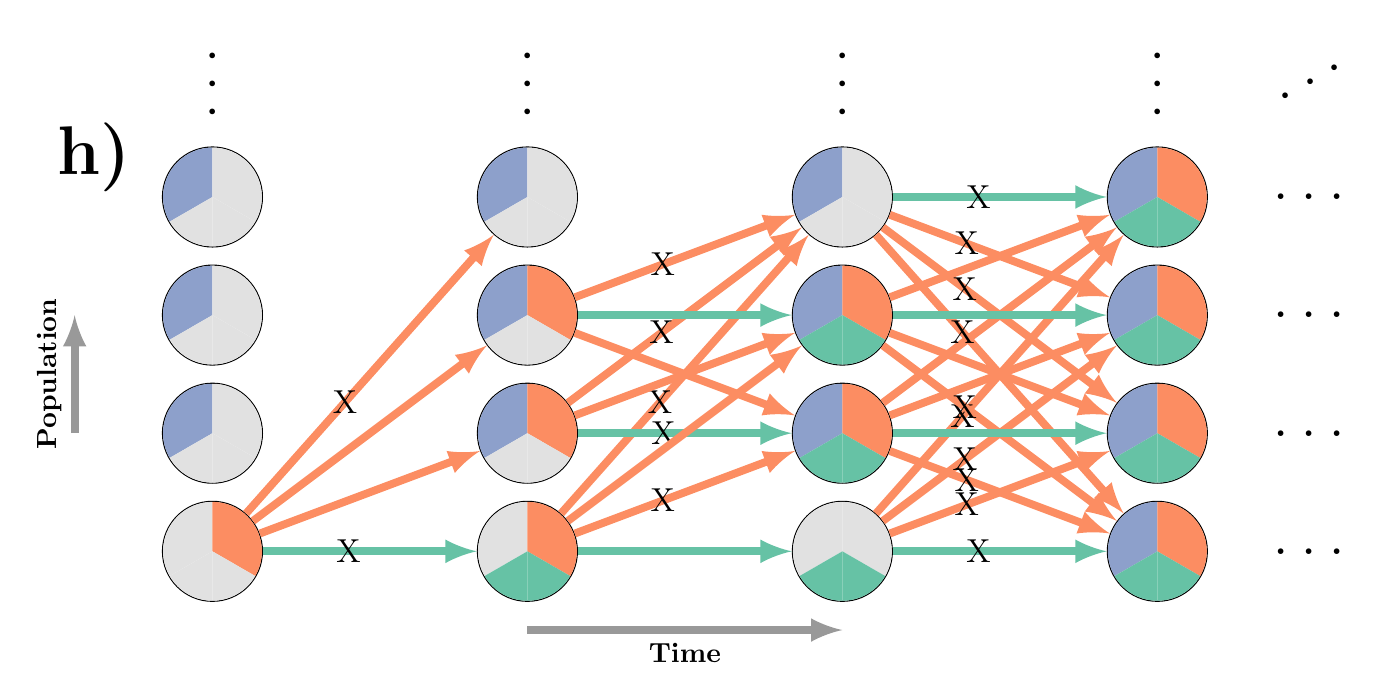
\begin{tikzpicture}
  \draw (-1.5,5) node {\Huge \textbf{h)}};
  \draw (0,0) node[node,circle tri split part fill={nothing,infection,nothing}] (P11) {};
  \draw (0,1.5) node[node,circle tri split part fill={susceptible,nothing,nothing}] (P21) {};
  \draw (0,3) node[node,circle tri split part fill={susceptible,nothing,nothing}] (P31) {};
  \draw (0,4.5) node[node,circle tri split part fill={susceptible,nothing,nothing}] (P41) {};

  \draw (4,0) node[node,circle tri split part fill={nothing,infection,recovery}] (P12) {};
  \draw (4,1.5) node[node,circle tri split part fill={susceptible,infection,nothing}] (P22) {};
  \draw (4,3) node[node,circle tri split part fill={susceptible,infection,nothing}] (P32) {};
  \draw (4,4.5) node[node,circle tri split part fill={susceptible,nothing,nothing}] (P42) {};

  \draw (8,0) node[node,circle tri split part fill={nothing,nothing,recovery}] (P13) {};
  \draw (8,1.5) node[node,circle tri split part fill={susceptible,infection,recovery}] (P23) {};
  \draw (8,3) node[node,circle tri split part fill={susceptible,infection,recovery}] (P33) {};
  \draw (8,4.5) node[node,circle tri split part fill={susceptible,nothing,nothing}] (P43) {};

  \draw (12,0) node[node,circle tri split part fill={susceptible,infection,recovery}] (P14) {};
  \draw (12,1.5) node[node,circle tri split part fill={susceptible,infection,recovery}] (P24) {};
  \draw (12,3) node[node,circle tri split part fill={susceptible,infection,recovery}] (P34) {};
  \draw (12,4.5) node[node,circle tri split part fill={susceptible,infection,recovery}] (P44) {};

  \draw[-latex,line width=1mm, color=infection] (P11) -- (P22);
  \draw[-latex,line width=1mm, color=infection] (P11) -- (P32);
  \draw[-latex,line width=1mm, color=infection] (P11) -- node[pos=.4,text=black]{\Leftscissor} (P42);
  
  \draw[-latex,line width=1mm, color=recovery] (P11) -- node[pos=.4,text=black]{\Leftscissor} (P12);
  
  \draw[-latex,line width=1mm, color=infection] (P12) -- node[pos=.4,text=black]{\Leftscissor} (P23);
  \draw[-latex,line width=1mm, color=infection] (P12) -- node[pos=.4,text=black]{\Leftscissor} (P43);
  \draw[-latex,line width=1mm, color=infection] (P22) -- node[pos=.4,text=black]{\Leftscissor} (P43);
  \draw[-latex,line width=1mm, color=infection] (P32) -- node[pos=.4,text=black]{\Leftscissor} (P43);
  \draw[-latex,line width=1mm, color=recovery] (P22) -- node[pos=.4,text=black]{\Leftscissor} (P23);

  \draw[-latex,line width=1mm, color=infection] (P12) -- (P33);
  \draw[-latex,line width=1mm, color=infection] (P22) -- (P33);
  \draw[-latex,line width=1mm, color=infection] (P32) -- (P23);
  
  \draw[-latex,line width=1mm, color=recovery] (P12) -- (P13);
  \draw[-latex,line width=1mm, color=recovery] (P32) -- (P33);
  
  \draw[-latex,line width=1mm, color=infection] (P13) -- node[pos=.35,text=black]{\Leftscissor} (P24);
  \draw[-latex,line width=1mm, color=infection] (P13) -- node[pos=.35,text=black]{\Leftscissor} (P34);
  \draw[-latex,line width=1mm, color=infection] (P13) -- node[pos=.35,text=black]{\Leftscissor} (P44);
  \draw[-latex,line width=1mm, color=infection] (P23) -- node[pos=.35,text=black]{\Leftscissor} (P14);
  \draw[-latex,line width=1mm, color=infection] (P23) -- (P34);
  \draw[-latex,line width=1mm, color=infection] (P23) -- (P44);
  \draw[-latex,line width=1mm, color=infection] (P33) -- node[pos=.35,text=black]{\Leftscissor} (P14);
  \draw[-latex,line width=1mm, color=infection] (P33) -- (P24);
  \draw[-latex,line width=1mm, color=infection] (P33) -- (P44);
  \draw[-latex,line width=1mm, color=infection] (P43) -- node[pos=.35,text=black]{\Leftscissor} (P14);
  \draw[-latex,line width=1mm, color=infection] (P43) -- node[pos=.35,text=black]{\Leftscissor} (P24);
  \draw[-latex,line width=1mm, color=infection] (P43) -- node[pos=.35,text=black]{\Leftscissor} (P34);
  
  \draw[-latex,line width=1mm, color=recovery] (P13) -- node[pos=.4,text=black]{\Leftscissor} (P14);
  \draw[-latex,line width=1mm, color=recovery] (P23) -- (P24);
  \draw[-latex,line width=1mm, color=recovery] (P33) -- (P34);
  \draw[-latex,line width=1mm, color=recovery] (P43) -- node[pos=.4,text=black]{\Leftscissor} (P44);

  %% Extends on
  \draw (14,0) node{\Huge \dots};
  \draw (14,1.5) node{\Huge \dots};
  \draw (14,3) node{\Huge \dots};
  \draw (14,4.5) node{\Huge \dots};

  \draw (0,6) node[rotate=90]{\Huge \dots};
  \draw (4,6) node[rotate=90]{\Huge \dots};
  \draw (8,6) node[rotate=90]{\Huge \dots};
  \draw (12,6) node[rotate=90]{\Huge \dots};
  \draw (14,6) node[rotate=30]{\Huge \dots};
  %% Legend things
  \draw[-latex,line width=1mm,white!60!black] (4,-1) -- (8,-1) node[midway, below,text=black] {\textbf{Time}};
  \draw[-latex,line width=1mm,white!60!black] (-1.75,1.5) -- (-1.75,3) node[midway, above,text=black,rotate=90] {\textbf{Population}};
\end{tikzpicture}

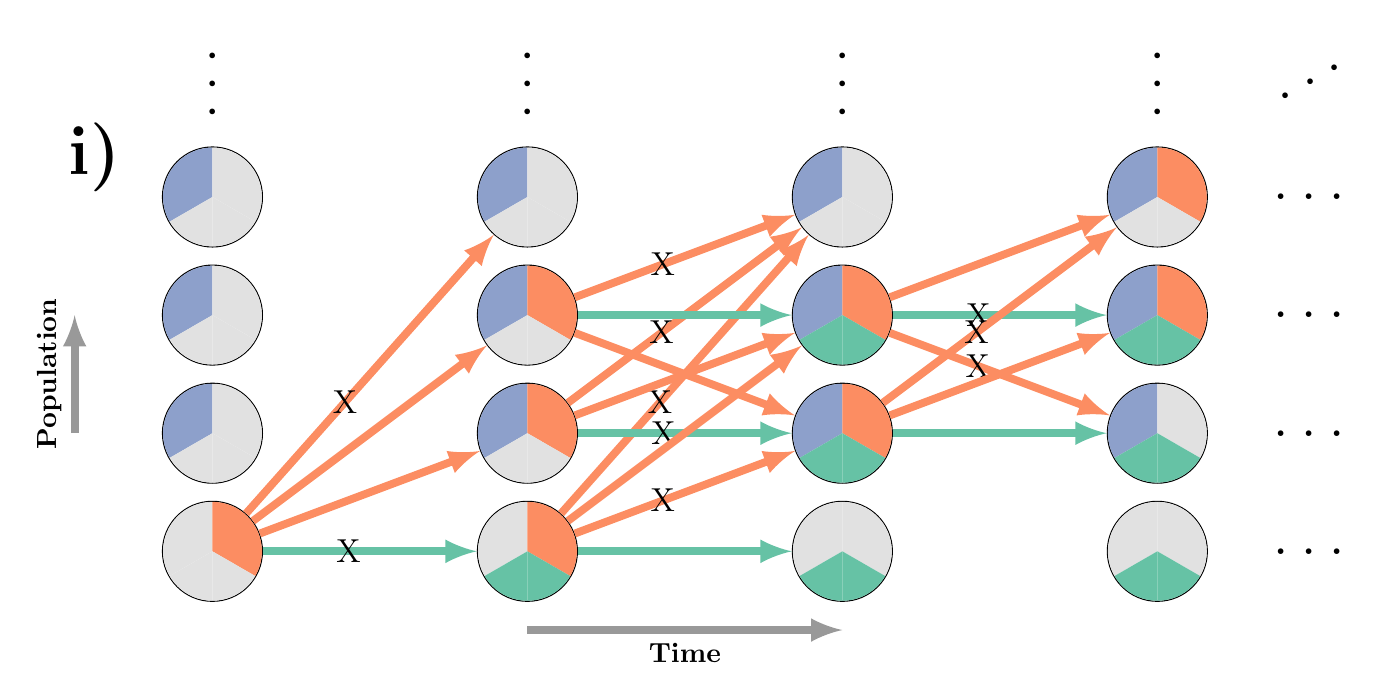
\begin{tikzpicture}
  \draw (-1.5,5) node {\Huge \textbf{i)}};
  \draw (0,0) node[node,circle tri split part fill={nothing,infection,nothing}] (P11) {};
  \draw (0,1.5) node[node,circle tri split part fill={susceptible,nothing,nothing}] (P21) {};
  \draw (0,3) node[node,circle tri split part fill={susceptible,nothing,nothing}] (P31) {};
  \draw (0,4.5) node[node,circle tri split part fill={susceptible,nothing,nothing}] (P41) {};

  \draw (4,0) node[node,circle tri split part fill={nothing,infection,recovery}] (P12) {};
  \draw (4,1.5) node[node,circle tri split part fill={susceptible,infection,nothing}] (P22) {};
  \draw (4,3) node[node,circle tri split part fill={susceptible,infection,nothing}] (P32) {};
  \draw (4,4.5) node[node,circle tri split part fill={susceptible,nothing,nothing}] (P42) {};

  \draw (8,0) node[node,circle tri split part fill={nothing,nothing,recovery}] (P13) {};
  \draw (8,1.5) node[node,circle tri split part fill={susceptible,infection,recovery}] (P23) {};
  \draw (8,3) node[node,circle tri split part fill={susceptible,infection,recovery}] (P33) {};
  \draw (8,4.5) node[node,circle tri split part fill={susceptible,nothing,nothing}] (P43) {};

  \draw (12,0) node[node,circle tri split part fill={nothing,nothing,recovery}] (P14) {};
  \draw (12,1.5) node[node,circle tri split part fill={susceptible,nothing,recovery}] (P24) {};
  \draw (12,3) node[node,circle tri split part fill={susceptible,infection,recovery}] (P34) {};
  \draw (12,4.5) node[node,circle tri split part fill={susceptible,infection,nothing}] (P44) {};

  \draw[-latex,line width=1mm, color=infection] (P11) -- (P22);
  \draw[-latex,line width=1mm, color=infection] (P11) -- (P32);
  \draw[-latex,line width=1mm, color=infection] (P11) -- node[pos=.4,text=black]{\Leftscissor} (P42);
  
  \draw[-latex,line width=1mm, color=recovery] (P11) -- node[pos=.4,text=black]{\Leftscissor} (P12);
  
  \draw[-latex,line width=1mm, color=infection] (P12) -- node[pos=.4,text=black]{\Leftscissor} (P23);
  \draw[-latex,line width=1mm, color=infection] (P12) -- node[pos=.4,text=black]{\Leftscissor} (P43);
  \draw[-latex,line width=1mm, color=infection] (P22) -- node[pos=.4,text=black]{\Leftscissor} (P43);
  \draw[-latex,line width=1mm, color=infection] (P32) -- node[pos=.4,text=black]{\Leftscissor} (P43);
  \draw[-latex,line width=1mm, color=recovery] (P22) -- node[pos=.4,text=black]{\Leftscissor} (P23);

  \draw[-latex,line width=1mm, color=infection] (P12) -- (P33);
  \draw[-latex,line width=1mm, color=infection] (P22) -- (P33);
  \draw[-latex,line width=1mm, color=infection] (P32) -- (P23);
  
  \draw[-latex,line width=1mm, color=recovery] (P12) -- (P13);
  \draw[-latex,line width=1mm, color=recovery] (P32) -- (P33);

  \draw[-latex,line width=1mm, color=recovery] (P33) --  node[pos=.4,text=black]{\Leftscissor} (P34);
  \draw[-latex,line width=1mm, color=infection] (P33) -- node[pos=.4,text=black]{\Leftscissor} (P24);
  \draw[-latex,line width=1mm, color=infection] (P23) -- node[pos=.4,text=black]{\Leftscissor} (P44);
  
  \draw[-latex,line width=1mm, color=infection] (P23) -- (P34);
  \draw[-latex,line width=1mm, color=infection] (P33) -- (P44);
  
  \draw[-latex,line width=1mm, color=recovery] (P23) -- (P24);

  %% Extends on
  \draw (14,0) node{\Huge \dots};
  \draw (14,1.5) node{\Huge \dots};
  \draw (14,3) node{\Huge \dots};
  \draw (14,4.5) node{\Huge \dots};

  \draw (0,6) node[rotate=90]{\Huge \dots};
  \draw (4,6) node[rotate=90]{\Huge \dots};
  \draw (8,6) node[rotate=90]{\Huge \dots};
  \draw (12,6) node[rotate=90]{\Huge \dots};
  \draw (14,6) node[rotate=30]{\Huge \dots};
  %% Legend things
  \draw[-latex,line width=1mm,white!60!black] (4,-1) -- (8,-1) node[midway, below,text=black] {\textbf{Time}};
  \draw[-latex,line width=1mm,white!60!black] (-1.75,1.5) -- (-1.75,3) node[midway, above,text=black,rotate=90] {\textbf{Population}};
\end{tikzpicture}

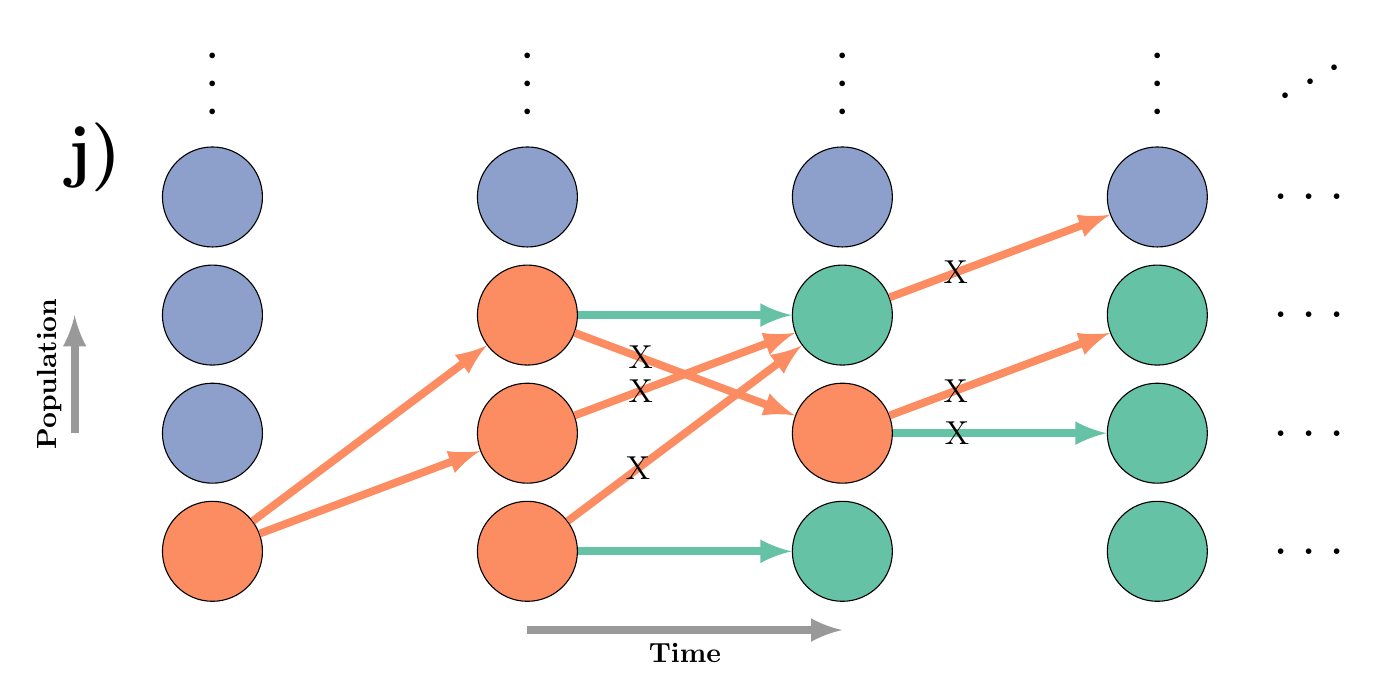
\begin{tikzpicture}
  \draw (-1.5,5) node {\Huge \textbf{j)}};
  \draw (0,0) node[node,circle,fill=infection] (P11) {};
  \draw (0,1.5) node[node,circle,fill=susceptible] (P21) {};
  \draw (0,3) node[node,circle,fill=susceptible] (P31) {};
  \draw (0,4.5) node[node,circle,fill=susceptible] (P41) {};

  \draw (4,0) node[node,circle,fill=infection] (P12) {};
  \draw (4,1.5) node[node,circle,fill=infection] (P22) {};
  \draw (4,3) node[node,circle,fill=infection] (P32) {};
  \draw (4,4.5) node[node,circle,fill=susceptible] (P42) {};

  \draw (8,0) node[node,circle,fill=recovery] (P13) {};
  \draw (8,1.5) node[node,circle,fill=infection] (P23) {};
  \draw (8,3) node[node,circle,fill=recovery] (P33) {};
  \draw (8,4.5) node[node,circle,fill=susceptible] (P43) {};

  \draw (12,0) node[node,circle,fill=recovery] (P14) {};
  \draw (12,1.5) node[node,circle,fill=recovery] (P24) {};
  \draw (12,3) node[node,circle,fill=recovery] (P34) {};
  \draw (12,4.5) node[node,circle,fill=susceptible] (P44) {};

  \draw[-latex,line width=1mm, color=infection] (P11) -- (P22);
  \draw[-latex,line width=1mm, color=infection] (P11) -- (P32);
  
  \draw[-latex,line width=1mm, color=infection] (P12) -- node[pos=.3,text=black]{\Leftscissor} (P33);
  \draw[-latex,line width=1mm, color=infection] (P22) -- node[pos=.3,text=black]{\Leftscissor} (P33);
  \draw[-latex,line width=1mm, color=infection] (P32) -- node[pos=.3,text=black]{\Leftscissor} (P23);
  
  \draw[-latex,line width=1mm, color=recovery] (P12) -- (P13);
  \draw[-latex,line width=1mm, color=recovery] (P32) -- (P33);

  \draw[-latex,line width=1mm, color=infection] (P23) -- node[pos=.3,text=black]{\Leftscissor} (P34);
  \draw[-latex,line width=1mm, color=infection] (P33) -- node[pos=.3,text=black]{\Leftscissor} (P44);
  
  \draw[-latex,line width=1mm, color=recovery] (P23) -- node[pos=.3,text=black]{\Leftscissor} (P24);

  %% Extends on
  \draw (14,0) node{\Huge \dots};
  \draw (14,1.5) node{\Huge \dots};
  \draw (14,3) node{\Huge \dots};
  \draw (14,4.5) node{\Huge \dots};

  \draw (0,6) node[rotate=90]{\Huge \dots};
  \draw (4,6) node[rotate=90]{\Huge \dots};
  \draw (8,6) node[rotate=90]{\Huge \dots};
  \draw (12,6) node[rotate=90]{\Huge \dots};
  \draw (14,6) node[rotate=30]{\Huge \dots};
  %% Legend things
  \draw[-latex,line width=1mm,white!60!black] (4,-1) -- (8,-1) node[midway, below,text=black] {\textbf{Time}};
  \draw[-latex,line width=1mm,white!60!black] (-1.75,1.5) -- (-1.75,3) node[midway, above,text=black,rotate=90] {\textbf{Population}};
\end{tikzpicture}

\begin{tikzpicture}
\draw[white](0,0) -- (1,1);
\end{tikzpicture}

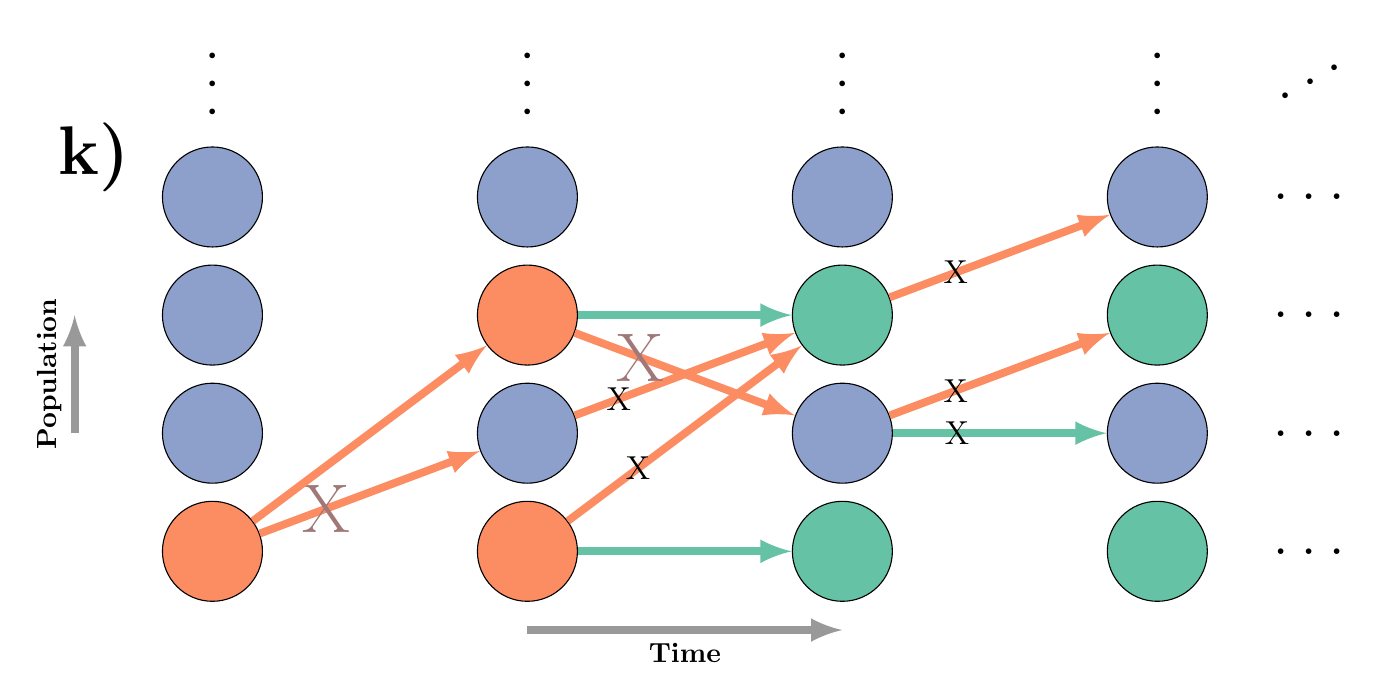
\begin{tikzpicture}
  \draw (-1.5,5) node {\Huge \textbf{k)}};
  \draw (0,0) node[node,circle,fill=infection] (P11) {};
  \draw (0,1.5) node[node,circle,fill=susceptible] (P21) {};
  \draw (0,3) node[node,circle,fill=susceptible] (P31) {};
  \draw (0,4.5) node[node,circle,fill=susceptible] (P41) {};

  \draw (4,0) node[node,circle,fill=infection] (P12) {};
  \draw (4,1.5) node[node,circle,fill=susceptible] (P22) {};
  \draw (4,3) node[node,circle,fill=infection] (P32) {};
  \draw (4,4.5) node[node,circle,fill=susceptible] (P42) {};

  \draw (8,0) node[node,circle,fill=recovery] (P13) {};
  \draw (8,1.5) node[node,circle,fill=susceptible] (P23) {};
  \draw (8,3) node[node,circle,fill=recovery] (P33) {};
  \draw (8,4.5) node[node,circle,fill=susceptible] (P43) {};

  \draw (12,0) node[node,circle,fill=recovery] (P14) {};
  \draw (12,1.5) node[node,circle,fill=susceptible] (P24) {};
  \draw (12,3) node[node,circle,fill=recovery] (P34) {};
  \draw (12,4.5) node[node,circle,fill=susceptible] (P44) {};

  \draw[-latex,line width=1mm, color=infection] (P11) -- node[pos=.3,text=intervention]{\Largescissor} (P22);
  \draw[-latex,line width=1mm, color=infection] (P11) -- (P32);
  
  \draw[-latex,line width=1mm, color=infection] (P12) --  node[pos=.3,text=black]{\Leftscissor} (P33);
  \draw[-latex,line width=1mm, color=infection] (P22) -- node[pos=.2,text=black]{\Leftscissor}  (P33);
  \draw[-latex,line width=1mm, color=infection] (P32) -- node[pos=.3,text=intervention]{\Largescissor} (P23);
  
  \draw[-latex,line width=1mm, color=recovery] (P12) -- (P13);
  \draw[-latex,line width=1mm, color=recovery] (P32) -- (P33);

  \draw[-latex,line width=1mm, color=infection] (P23) --  node[pos=.3,text=black]{\Leftscissor} (P34);
  \draw[-latex,line width=1mm, color=infection] (P33) --  node[pos=.3,text=black]{\Leftscissor} (P44);
  
  \draw[-latex,line width=1mm, color=recovery] (P23) -- node[pos=.3,text=black]{\Leftscissor}  (P24);

  %% Extends on
  \draw (14,0) node{\Huge \dots};
  \draw (14,1.5) node{\Huge \dots};
  \draw (14,3) node{\Huge \dots};
  \draw (14,4.5) node{\Huge \dots};

  \draw (0,6) node[rotate=90]{\Huge \dots};
  \draw (4,6) node[rotate=90]{\Huge \dots};
  \draw (8,6) node[rotate=90]{\Huge \dots};
  \draw (12,6) node[rotate=90]{\Huge \dots};
  \draw (14,6) node[rotate=30]{\Huge \dots};
  %% Legend things
  \draw[-latex,line width=1mm,white!60!black] (4,-1) -- (8,-1) node[midway, below,text=black] {\textbf{Time}};
  \draw[-latex,line width=1mm,white!60!black] (-1.75,1.5) -- (-1.75,3) node[midway, above,text=black,rotate=90] {\textbf{Population}};
\end{tikzpicture}
\end{document}
